We initially tried to obtain a Frobenius relative-error guarantee by using \RPCholesky\ as a column Nystr\"om method. Given a dataset $D=\{\bx_1,\ldots,\bx_n\}$, the associated Gaussian kernel matrix is
\[
    \bK(i,j)=\exp\left(-\frac{1}{2\sigma}\|\bx_i-\bx_j\|^2\right),
\]
where $\sigma>0$ is the kernel bandwidth. The experiments below use our independent Python implementation, available at \href{\GitHubURL}{\GitHubURL}.

We first reproduce a subset of rows from Table 1 of \cite{chen_randomly_2025}, which compares \RPCholesky\ against greedy pivot selection and the optimal rank-$k$ approximation. We then repeat the same comparison for the Frobenius norm. For a low-rank approximation $\hat\bA$, define the relative trace and Frobenius errors by
\[
    \eta_{*}=\frac{\tr(\bA-\hat\bA)}{\tr(\bA)}
    \qquad\qquad
    \eta_F=\frac{\|\bA-\hat\bA\|_F}{\|\bA\|_F}.
\]
Table~\ref{tab:rel-error1000} reports these errors for rank $1000$ approximations. The ``Opt'' columns represent the error of the optimal rank-1000 approximation given by the truncated svd.

\begin{table}[H]
\centering
\begin{adjustbox}{max width=\textwidth}
\begin{tabular}{wl{3.6cm}cccccc}
\toprule
dataset & & $\eta_\ast$ & & & $\eta_F$ & \\
\cmidrule(lr){2-4}
\cmidrule(lr){5-7}
& Greedy & \RPCholesky & Opt & Greedy & \RPCholesky & Opt \\
\midrule
yolanda & 2.07e-1 & \textbf{1.40e-1} & 8.71e-2 & 4.64e-2 & \textbf{6.30e-3} & 3.15e-3 \\
mnist\_784 & 1.70e-1 & \textbf{1.09e-1} & 5.96e-2 & 2.53e-2 & \textbf{4.95e-3} & 1.97e-3 \\
jannis & 1.27e-1 & \textbf{1.09e-1} & 5.42e-2 & 1.16e-2 & \textbf{6.52e-3} & 2.16e-3 \\
volkert & 6.09e-2 & \textbf{4.31e-2} & 2.06e-2 & 8.15e-3 & \textbf{2.26e-3} & 7.16e-4 \\
creditcard & 4.36e-2 & \textbf{2.32e-2} & 9.87e-3 & 1.04e-2 & \textbf{1.60e-3} & 5.04e-4 \\
hls4ml\_lhc\_jets\_hlf & 6.62e-5 & \textbf{4.47e-5} & 1.07e-5 & 1.27e-5 & \textbf{4.77e-6} & 7.97e-7 \\
\bottomrule
\end{tabular}
\end{adjustbox}
\caption{Relative trace and Frobenius errors of rank-1000 greedy and \RPCholesky\ methods when used to approximate a Gaussian kernel matrix. Each dataset is pruned to $10^4$ points and standardized, and we report the median across 10 trials. The error of the optimal rank-1000 approximation is included for reference.}
\label{tab:rel-error1000}
\end{table}

The table suggests that \RPCholesky\ performs well on these kernel matrices in both norms. It consistently improves over greedy pivot selection and is often within a small constant factor of the optimal rank-$1000$ error. This empirical behavior was the original motivation for asking whether \RPCholesky\ might satisfy a Frobenius relative-error guarantee analogous to its trace-error guarantee.

\begin{figure}[H]
    \centering
    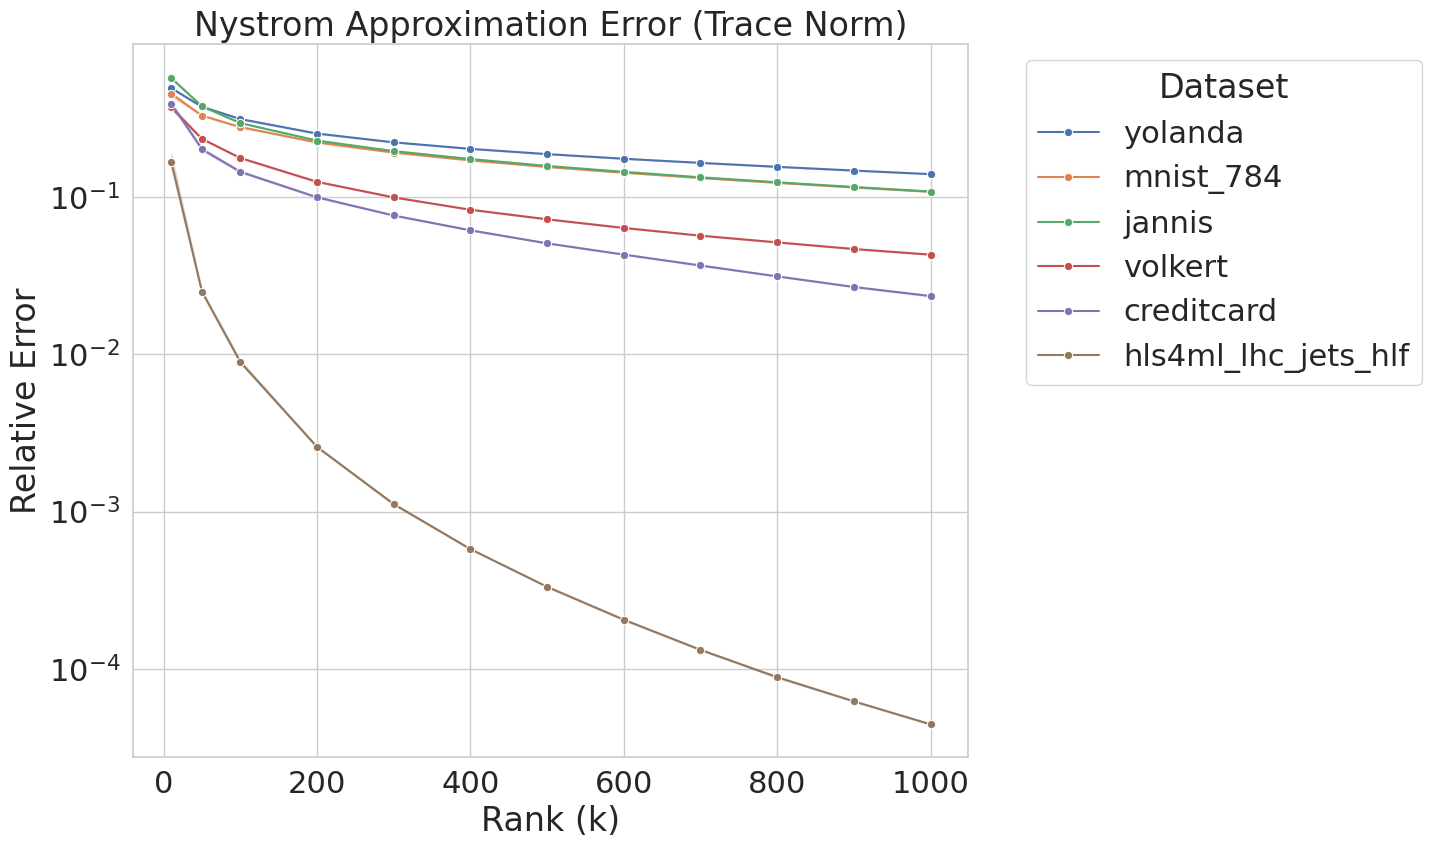
\includegraphics[width=0.8\linewidth]{images/rpcholesky_tr_error.png}
    \caption{Relative trace error vs approximation rank when \RPCholesky\ is used to approximate a Gaussian kernel matrix. Each dataset is trimmed to $10^4$ points and standardized. The bandwidth is set to $\sigma=\sqrt d$ for each dataset, where $d$ is the number of features. The plot depicts the mean and 95\% confidence interval across 10 trials for each value of $k$.}
    \label{fig:rpcholesky_rel_tr}
\end{figure}

\begin{figure}[H]
    \centering
    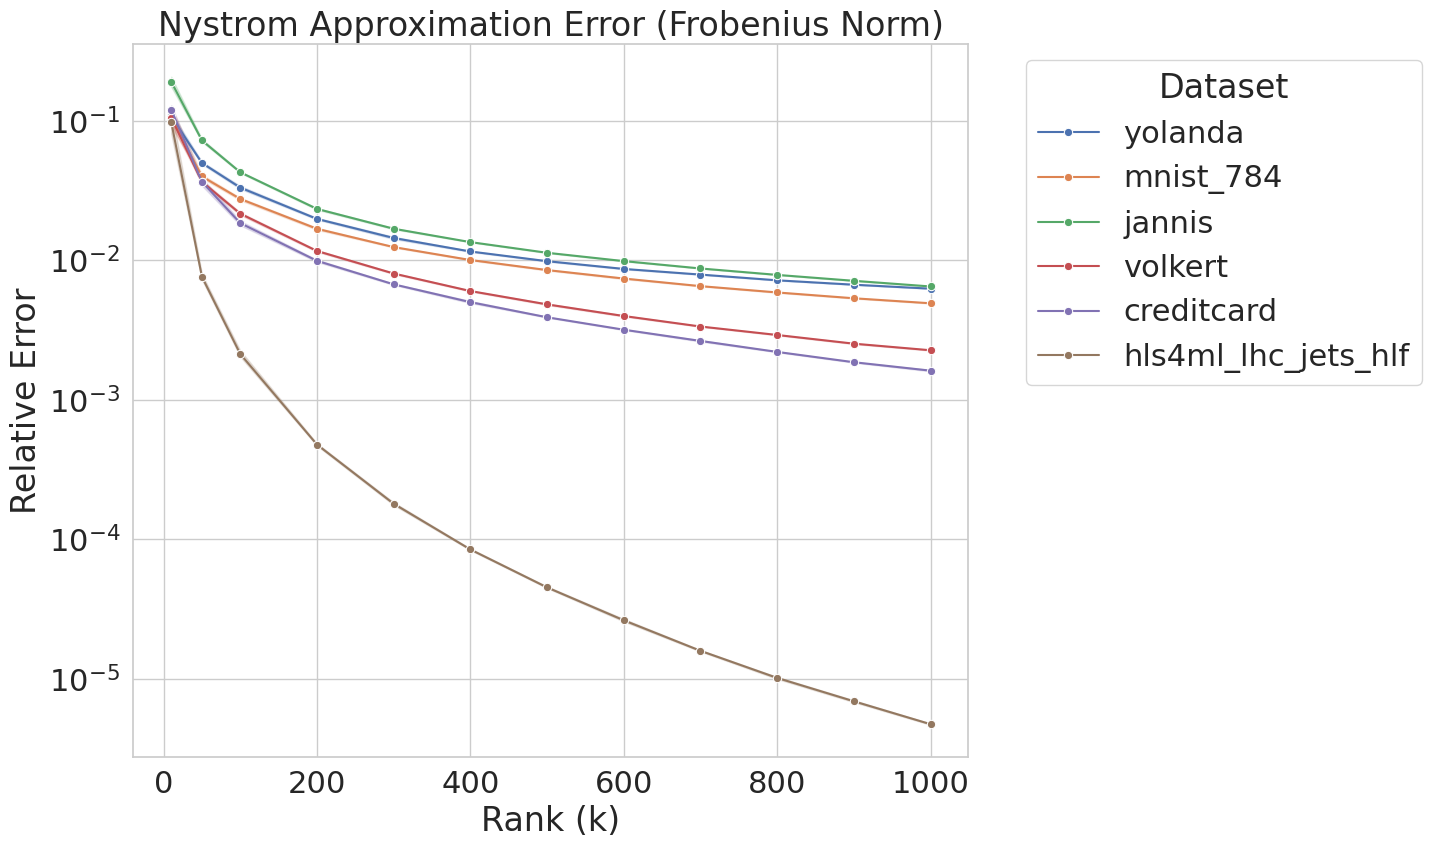
\includegraphics[width=0.8\linewidth]{images/rpcholesky_fro_error.png}
    \caption{Relative Frobenius error vs approximation rank when \RPCholesky\ is used to approximate a Gaussian kernel matrix. Each dataset is trimmed to $10^4$ points and standardized. The bandwidth is set to $\sigma=\sqrt d$ for each dataset, where $d$ is the number of features. The plot depicts the mean and 95\% confidence interval across 10 trials for each value of $k$.}
    \label{fig:rpcholesky_rel_fro}
\end{figure}

\begin{figure}[H]
    \centering
    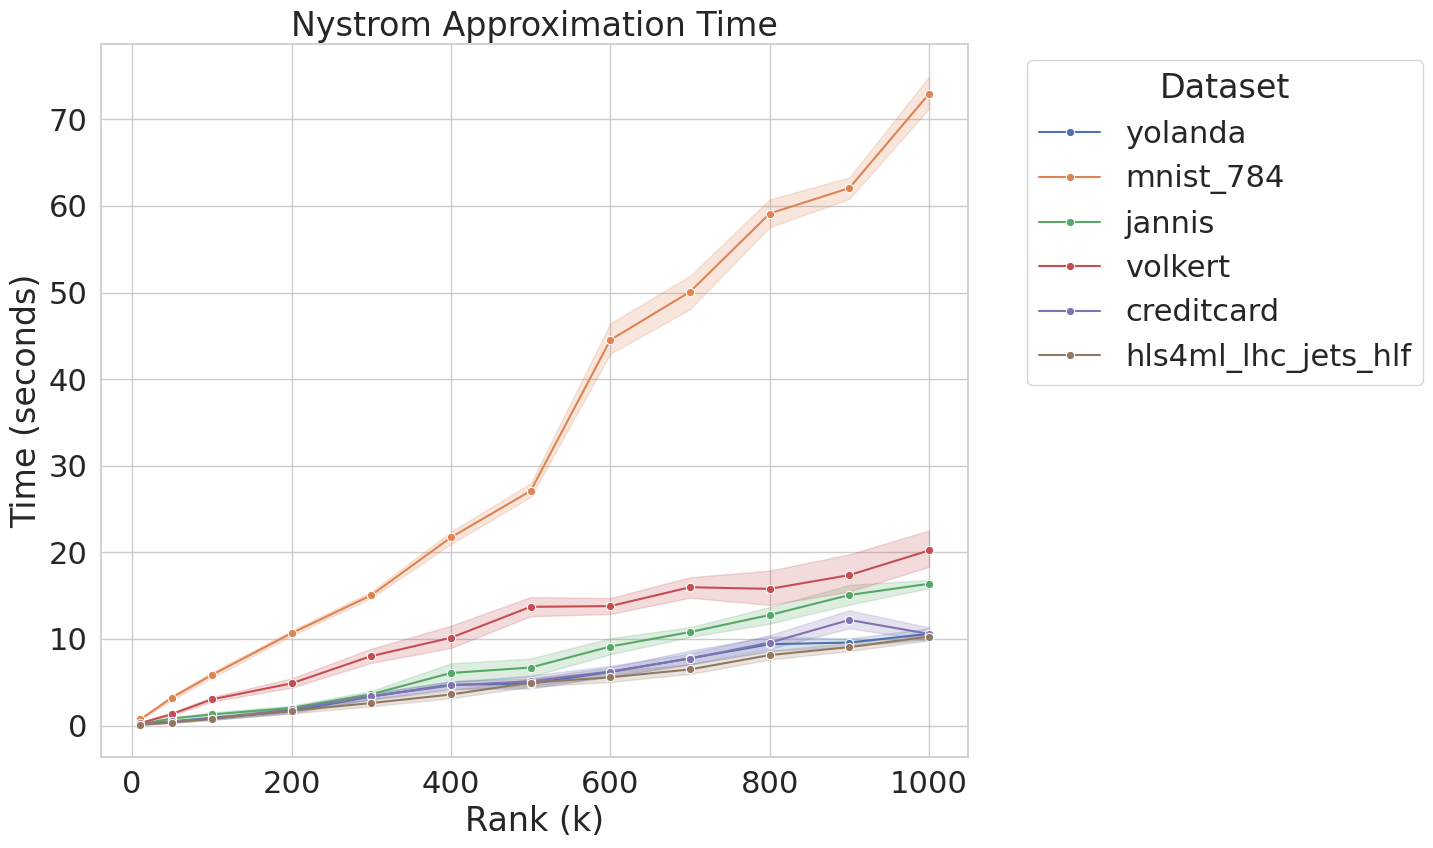
\includegraphics[width=0.8\linewidth]{images/rpcholesky_time.png}
    \caption{Computation time vs approximation rank when \RPCholesky\ is used to approximate a Gaussian kernel matrix. Each dataset is trimmed to $10^4$ points and standardized. The bandwidth is set to $\sigma=\sqrt d$ for each dataset, where $d$ is the number of features. The plot depicts the mean and 95\% confidence interval across 10 trials for each value of $k$.}
    \label{fig:rpcholesky_time}
\end{figure}

Figures~\ref{fig:rpcholesky_rel_tr} and~\ref{fig:rpcholesky_rel_fro} show that the relative error decays steadily as the approximation rank increases. The rate of decay varies substantially across datasets, which reflects differences in the spectra of the corresponding kernel matrices. Figure~\ref{fig:rpcholesky_time} shows approximately increasing runtime as a function of $k$. The cost of each entry query depends on the ambient feature dimension of the dataset; hence, the running time varies between datasets.

The preceding comparison measures error relative to $\|\bA\|_F^2$ or $\tr(\bA)$ rather than relative to the optimal residual. To probe relative-error behavior more directly, fix a target rank $r$ and an index set $S$, and define the trace and Frobenius residual ratios
\[
    \gamma_{r,*}(S)=
    \frac{\tr(\bA-\bA\gen{S})}{\tr(\bA-\bA_r)},
    \qquad
    \gamma_{r,F}(S)=
    \frac{\|\bA-\bA\gen{S}\|_F^2}{\|\bA-\bA_r\|_F^2}.
\]
For each $r$, each error measure, and each column-selection rule, we estimate the smallest Nystr\"om rank $k$ needed to match the optimal rank-$r$ error:
\[
    \min\{k\geq 1:\ \E[\gamma_{r,\bullet}(S)]\leq 1\},
\]
where $\bullet\in\{*,F\}$. The expectation is over the randomized column-selection procedure. Figure~\ref{fig:k-vs-r} reports this quantity for \RPCholesky\ and greedy selection on the \texttt{yolanda} dataset. For \RPCholesky, a larger approximation rank $k$ is required to match the optimal rank-$r$ approximation in the Frobenius norm compared to the trace norm.

\begin{figure}[H]
    \centering
    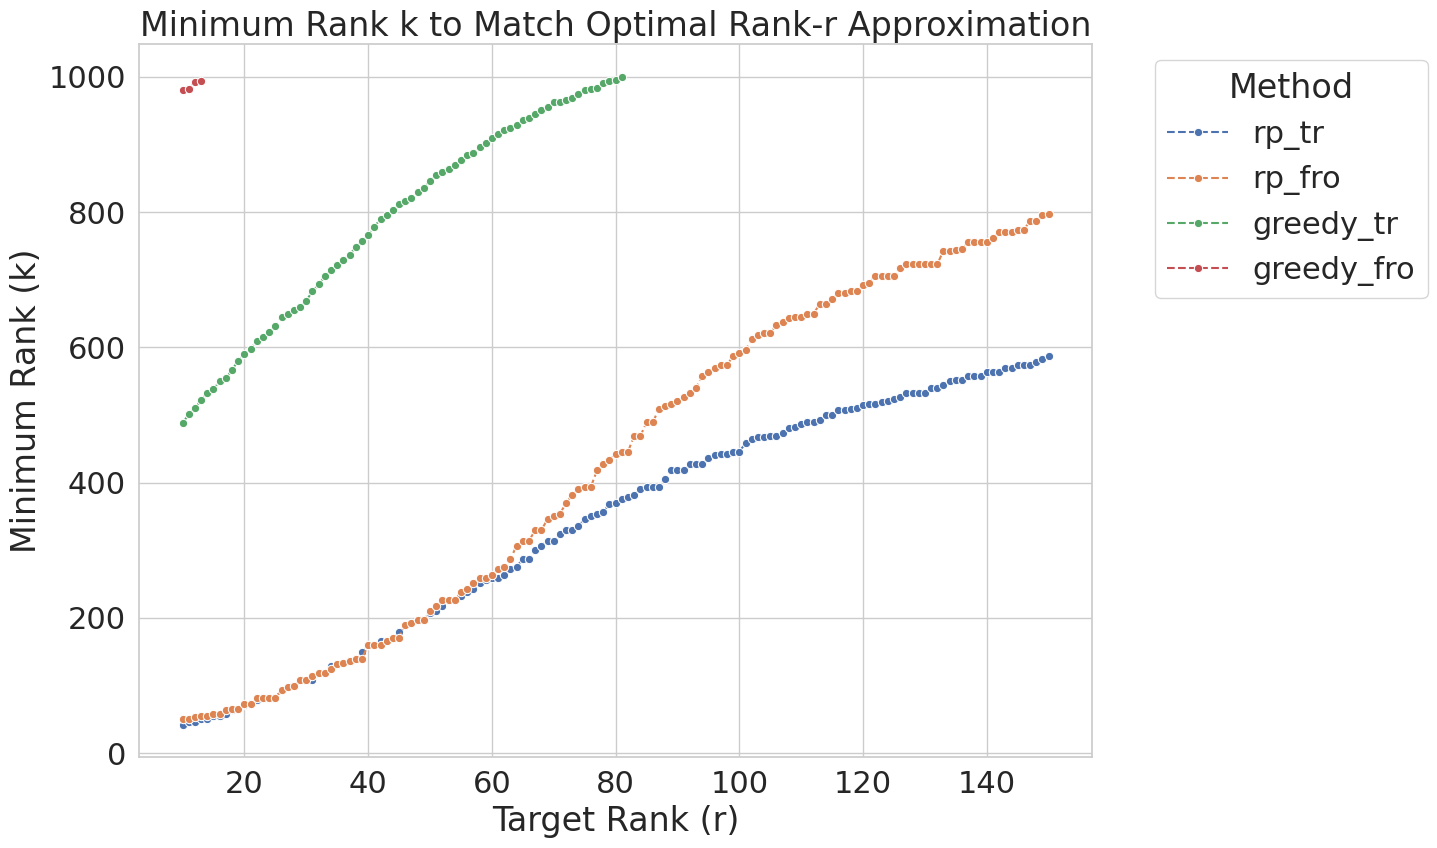
\includegraphics[width=0.98\linewidth]{images/min_k_to_opt_r_threshold1.png}
    \caption{Smallest Nystr\"om approximation rank $k$ required to match optimal rank-$r$ approximation error on the \texttt{yolanda} dataset. The plotted methods compare \RPCholesky\ and greedy pivot selection under trace and Frobenius error.}
    \label{fig:k-vs-r}
\end{figure}

The empirical results make \RPCholesky\ a natural first candidate for Frobenius relative-error approximation. Nevertheless, this direction fails in the worst case. The following construction shows that \RPCholesky\ can miss columns with large Frobenius mass with high probability. A related result appears in \cite[Section~11.2]{epperly_make_2025}, but we present the proof below to document a specific hard matrix for \RPCholesky.

\begin{theorem}
    \label{thm:rpc-frobenius-error-lower-bound}
    Fix $r\in\N$ and $c\geq 1$. For all sufficiently large $n$, there is a psd matrix $\bA\in\R^{n\times n}$ for which the Nystr\"om approximation $\bA\gen{S}$ produced by \RPCholesky\ satisfies
    \[
        \E\left[\|\bA-\bA\gen{S}\|_F^2\right]
        > c\cdot \|\bA-\bA_r\|_F^2
    \]
    for all $|S|<\sqrt n/(4c)$.
\end{theorem}

\begin{proof}
    We produce $\bA$ directly. Consider the matrix

    \begin{equation} 
    \label{eq:rpcholesky-worst-case}
    \bA = 
    \begin{pmatrix}
        \underbrace{\begin{matrix}
        1 & \cdots & 1 \\
        \vdots& \ddots &\vdots\\
        1 & \cdots & 1 \\
        \end{matrix}}_{\text{$m$}}\\
        && 1 & \\
        && & \ddots \\
        && & & 1 \\
    \end{pmatrix}
    \end{equation}

    The optimal rank-1 approximation is spanned by any of the first $m$ columns of $\bA$, with error 
    \[\delta := \|\bA - \bA_1\|^2_F = n-m.\]
    
   Suppose \RPCholesky\ selects $k$ columns. The diagonal entries of $\bA$ have equal weight, so \RPCholesky\ chooses each column with equal probability. The number of optimal columns selected by \RPCholesky\ follows a hypergeometric distribution, 
   \[X\sim\Hypergeometric(n,m,k).\]
   In particular, the probability that none of the optimal columns are chosen is
   \[
       p := \Pr[X = 0] = \prod_{i=0}^{k-1}\left(1-\frac{m}{n-i}\right).
   \]

   We obtain a lower bound for $p$ as follows:
    \begin{align*}
        p &= \prod_{i=0}^{k-1}\left(1-\frac{m}{n-i}\right)\\
        &= \exp\left(\sum_{i=0}^{k-1}\log\left(1-x_i\right)\right)\qquad x_i=\frac{m}{n-i} \in (0, 1)\\
        &\geq \exp\left(-\sum_{i=0}^{k-1}\frac{m}{n-m-i}\right)\qquad\text{using $\log(1-x_i)\geq -\frac{x_i}{1-x_i}$}\\
        &\geq \exp\left(-\frac{km}{n-m-k}\right).
    \end{align*}
    If in addition we have $k < \sqrt{n}/(4c)$ and $m = c\sqrt{n}$, then 
    \begin{align*}
        n-m-k&\geq n-2m\\
        &\geq \frac{n}{2}\qquad\text{for $n\geq 16c^2$}
    \end{align*}
    and hence
    \begin{align*}
        p &\geq \exp\left(-\frac{km}{n-m-k}\right)\\
        &\geq \exp\left(-1/2\right)\\
        & > 1/2.
    \end{align*}
    
    By inspection, we see that the error of the rank-$k$ \RPCholesky\ approximation satisfies
   \[\|\bA - \bA\gen{S}\|^2_F\geq \begin{cases}
       m^2 +\delta-k&\text{with probability $p$}\\
       \delta-k+1 &\text{with probability $1-p.$}
   \end{cases}\]

   Thus,
   \begin{align*}
       \E\left[\|\bA - \bA\gen{S}\|^2_F\right]&\geq p(m^2+\delta-k)\\
       &> \frac{1}{2}\cdot \left(c^2n-k+\delta\right)\\
       &\geq \frac{1}{2}\cdot \delta(c^2+1)\\
       & \geq c\cdot \delta \qquad\text{for all $c\geq 1$}\\
       & \geq c\cdot \|\bA - \bA_r\|^2_F.
   \end{align*}

    Choosing $n$ large enough so that 
    \[n\geq 16c^2\]
    completes the proof.
    % where each $\bJ$ is the $\sqrt{n}\times \sqrt{n}$ all-ones matrix.
\end{proof}

The matrix in~\eqref{eq:rpcholesky-worst-case} has a simple geometric interpretation. Form a dataset with $N$ points in dimension $d$ by taking
\begin{enumerate}[
    label=\arabic*.,
    leftmargin=2em,
    itemsep=0.35em,
    topsep=0.45em,
    parsep=0pt
]
    \item $c\sqrt N$ points drawn from a spherical Gaussian distribution centered at the origin with covariance matrix $p\bI$, and
    \item $N-c\sqrt N$ points corresponding to vertices of the $d$-dimensional hypercube of width $2$ centered at the origin.
\end{enumerate}
The Gaussian kernel matrix of this dataset resembles the hard matrix above: the clustered points form a dense all-ones-like block, while the separated hypercube points contribute the diagonal block. Figure~\ref{fig:geom-hard} illustrates this structure.

\begin{figure}[H]
    \centering
    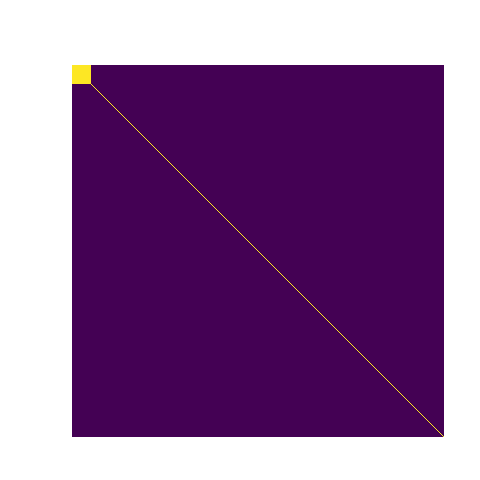
\includegraphics[width=0.60\linewidth]{images/rpcholesky_hard_matrix_c5_p0.0001_kernel_heatmap.png}
    \caption{Heatmap of the Gaussian kernel matrix for the geometric hard dataset at $N=10^4$, $d=100$, and $c=500$.}
    \label{fig:geom-hard}
\end{figure}

The preceding example suggests a natural modification of the pivot rule. The failure occurs because diagonal-proportional sampling treats the dense block and the isolated diagonal columns as equally important, even though the dense block contains much more Frobenius mass. A possible remedy is to sample a moderately large candidate principal submatrix, reweight it by the sampling probabilities, and then choose the candidate whose normalized sampled column appears largest. Taking $s\asymp \sqrt n$ candidates gives a constant probability of seeing a hidden block of size $\asymp\sqrt n$, after which the largest-column rule is designed to favor that block over the isolated columns.

\begin{algorithm}[H]
\caption{\RPCholesky2\ pivot selection}
\label{alg:rpc2}

\textbf{Input:} residual matrix \(\bR=\bA-\hat\bA\), parameter \(c>0\).
\smallskip

\begin{enumerate}[
    label=\arabic*.,
    leftmargin=2em,
    itemsep=0.35em,
    topsep=0.45em,
    parsep=0pt
]
    \item Define \(p_i=\bR_{ii}/\tr(\bR)\) and set \(s=\lceil c\sqrt n\rceil\).
    \item Draw candidate indices \(J=(j_1,\ldots,j_s)\) independently from the distribution \(p\).
    \item Form
    \[
        \bD=\diag(p_{j_1}^{-1/2},\ldots,p_{j_s}^{-1/2}),
        \qquad
        \bM=\bD\bR(J,J)\bD.
    \]
    \item Return \(j_{\ell^\star}\), where
    \[
        \ell^\star\in\argmax_{\ell\in[s]}
        \|\bM\bar{\mathbf m}_\ell\|_2^2,
        \qquad
        \bar{\mathbf m}_\ell=\frac{\bM_{:,\ell}}{\|\bM_{:,\ell}\|_2}.
    \]
\end{enumerate}
\end{algorithm}

The experiments below test this modified pivot rule on the same \texttt{yolanda} kernel matrix used in Figure~\ref{fig:k-vs-r}. Figure~\ref{fig:rpc2-vs-rpc} compares the smallest Nystr\"om rank $k$ required to match the optimal rank-$r$ error for \RPCholesky\ and \RPCholesky2, again under both trace and Frobenius errors. The modified rule reduces the required rank over much of the plotted range, but the improvement is empirical and does not by itself suggest a worst-case guarantee.

\begin{figure}[H]
    \centering
    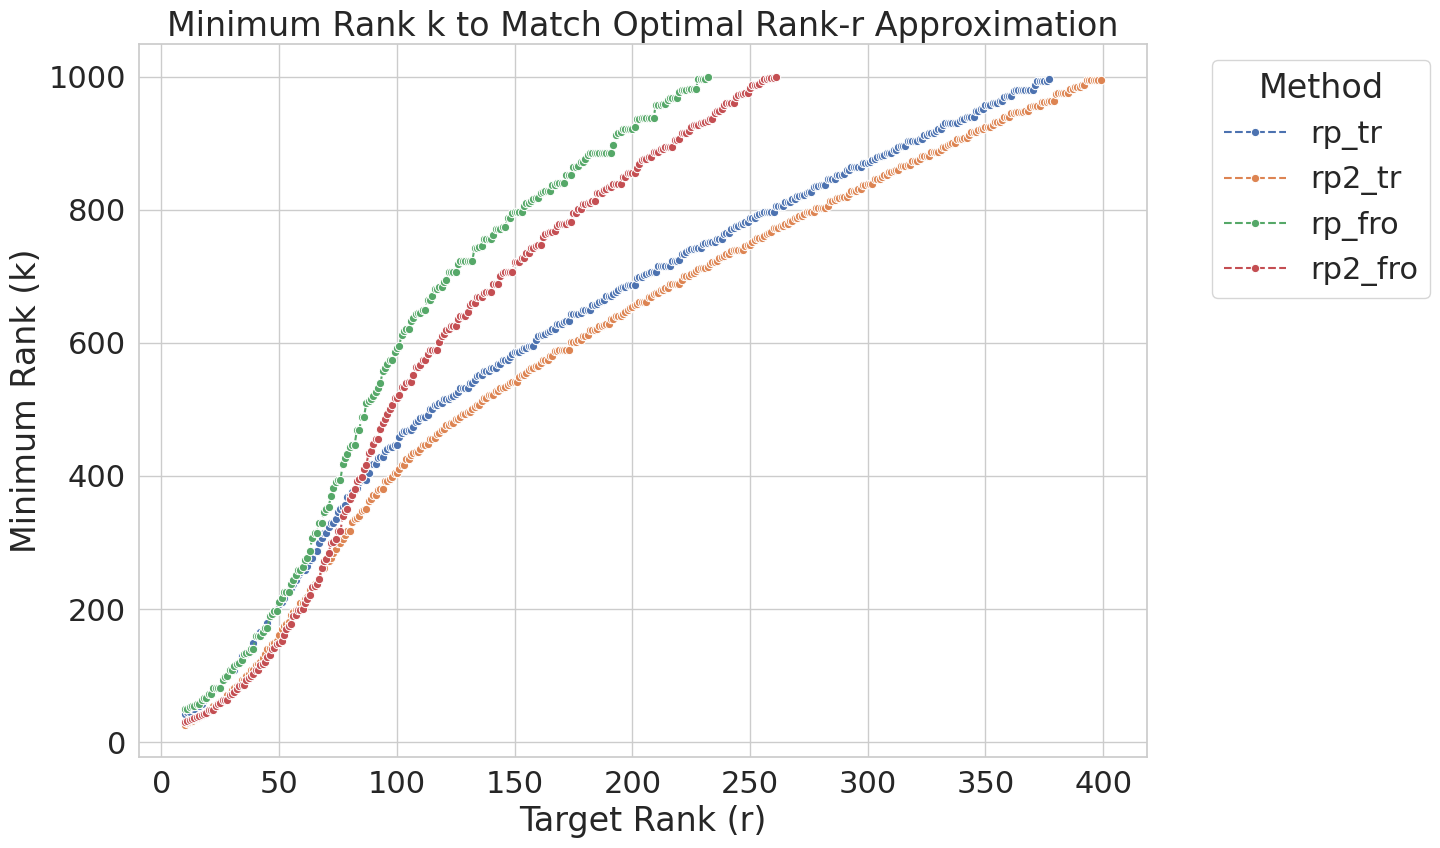
\includegraphics[width=0.90\linewidth]{images/min2_k_to_opt_r_threshold1.png}
    \caption{Smallest Nystr\"om approximation rank $k$ required to match the optimal rank-$r$ error on the \texttt{yolanda} dataset. The figure compares \RPCholesky\ and \RPCholesky2 under trace and Frobenius error.}
    \label{fig:rpc2-vs-rpc}
\end{figure}

Table~\ref{tab:rpc2-rel-error1000} compares rank-$1000$ \RPCholesky2\ and \RPCholesky\ approximations on the same benchmark datasets as Table~\ref{tab:rel-error1000}. The modified rule gives modest but consistent improvements in these tests. This is useful as a diagnostic, but the gains are not large enough to overcome the theoretical obstruction below.

\begin{table}[H]
\centering
\begin{adjustbox}{max width=\textwidth}
\begin{tabular}{wl{3.6cm}cccccc}
\toprule
dataset & & $\eta_\ast$ & & & $\eta_F$ & \\
\cmidrule(lr){2-4}
\cmidrule(lr){5-7}
& \RPCholesky2 & \RPCholesky & Opt & \RPCholesky2 & \RPCholesky & Opt \\
\midrule
yolanda & \textbf{1.38e-1} & 1.40e-1 & 8.71e-2 & \textbf{6.02e-3} & 6.30e-3 & 3.15e-3 \\
mnist\_784 & \textbf{1.04e-1} & 1.09e-1 & 5.96e-2 & \textbf{4.67e-3} & 4.95e-3 & 1.97e-3 \\
jannis & \textbf{1.07e-1} & 1.09e-1 & 5.42e-2 & \textbf{6.27e-3} & 6.52e-3 & 2.16e-3 \\
volkert & \textbf{4.07e-2} & 4.31e-2 & 2.06e-2 & \textbf{2.09e-3} & 2.26e-3 & 7.16e-4 \\
creditcard & \textbf{2.08e-2} & 2.32e-2 & 9.87e-3 & \textbf{1.39e-3} & 1.60e-3 & 5.04e-4 \\
hls4ml\_lhc\_jets\_hlf & \textbf{3.98e-5} & 4.47e-5 & 1.07e-5 & \textbf{4.01e-6} & 4.77e-6 & 7.97e-7 \\
\bottomrule
\end{tabular}
\end{adjustbox}
\caption{Relative trace and Frobenius error comparison between rank-1000 \RPCholesky\ and \RPCholesky2 methods when used to approximate a Gaussian kernel matrix. Each dataset is pruned to $10^4$ points and standardized, and we report the median across 10 trials. The error of the optimal rank-1000 approximation is included for reference.}
\label{tab:rpc2-rel-error1000}
\end{table}

Figure~\ref{fig:rpc2-c} shows the effect of the oversampling parameter $c$ on the \texttt{yolanda} dataset. Larger values of $c$ inspect larger candidate principal submatrices at each step, increasing the cost per pivot but improving the chance of identifying a high-Frobenius-mass column. 

\begin{figure}[H]
    \centering
    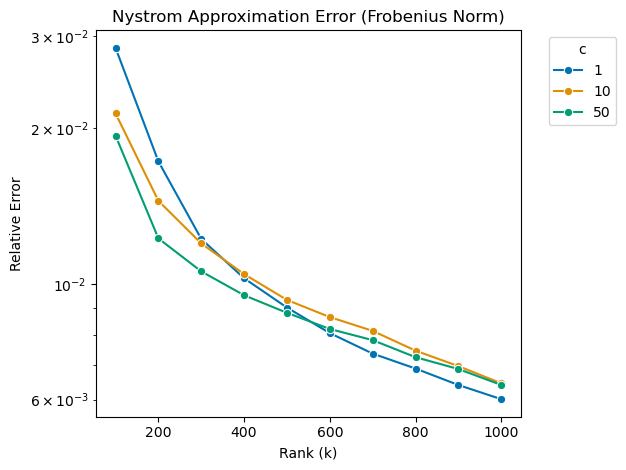
\includegraphics[width=0.75\linewidth]{images/rpc3_yolanda_fro_error_c.png}
    \caption{Relative Frobenius error of \RPCholesky2\ on the \texttt{yolanda} dataset with varied choices of $c$, where $c\sqrt n$ is the number of candidate indices used to form the sampled principal submatrix at each pivot step.}
    \label{fig:rpc2-c}
\end{figure}

We now introduce the main negative result of this section, which shows that $\Omega(\sqrt n)$ sampled columns are needed in the worst case to achieve a relative Frobenius error guarantee using the Nystr\"om approximation. We note that a similar lower bound appears in \cite{wang_improving_2013}. 

After querying the sampled columns, $\Omega(n^{1.5})$ entry queries are needed for a relative Frobenius error approximation. In particular, we cannot hope to achieve linear dependence on $n$, matching the results of \cite{musco_sublinear_2019, bakshi_robust_2020}, using a Nystr\"om approximation. 

\begin{theorem}[Nystr\"om lower bound]
    \label{thm:nystrom-frobenius-lb}
     For all $\alpha \geq 1$, there exist PSD matrices $\bA\in\R^{n\times n}$ such that \textbf{any} rank-$k$ column Nystr\"om approximation with 
    \[ k \leq \sqrt{n/(2\alpha)}\]
    has error $\|\bA - \bA\gen{S}\|^2_F > \alpha\cdot \|\bA - \bA_1\|^2_F$.
\end{theorem}


\begin{proof}
Let $\bA = \bI_n + \delta\bJ_n$ for some $\delta \geq 1$, where $\bI_n$ is the $n\times n$ identity matrix and $\bJ_n$ is the $n\times n$ all-ones matrix. The eigenvalues of $\bA$ are 
\[\lambda_1 = 1+n\delta \qquad \lambda_2 = 1\qquad\cdots\qquad \lambda_n = 1.\]
The first eigenvector of $\bA$ is $\bu_1 = (1/\sqrt n)\mathbf{1}$, and the best rank-1 approximation to $\bA$ is therefore given by
\[\bA_1 = (1 + n\delta)\bu_1\bu_1^\top = \left(\frac{1}{n}+\delta\right)\bJ_n \qquad 1 + n\delta \geq 1\]
with approximation error
\begin{align*}
    \|\bA - \bA_1\|^2_F = \sum_{i=2}^n\lambda_i^2 =n-1.\tag{$\ast$}
\end{align*}

On the other hand, suppose we choose $k$ columns of $\bA$ to compute the Nystr\"om approximation $\bA\gen{S}$. Without loss of generality, we can take the first $k$ columns, i.e., set $S = [k]$. With $d = n-k$, partition $\bA$ into blocks as follows:
\[\bA = \begin{pmatrix}
    \bA_{kk} & \bA_{kd}\\
    \bA_{dk} & \bA_{dd}
\end{pmatrix}\]
where 
\[\bA_{kk} = \bI_k + \delta\bJ_k\qquad \bA_{dk} = \bA_{kd}^\top = \delta\mathbf{1}_{d\times k}\qquad \bA_{dd} = \bI_d + \delta\bJ_d.\]

\vspace{1em}
The Nystr\"om approximation in block form is given by
\[\bA\gen{S} = \begin{pmatrix}
    \bA_{kk}\\
    \bA_{dk}
\end{pmatrix} \bA_{kk}^{-1}\begin{pmatrix}
    \bA_{kk}\\
    \bA_{dk}
\end{pmatrix}^\top = \begin{pmatrix}
    \bA_{kk} & \bA_{kd}\\
    \bA_{dk} & \bA_{dk}\bA_{kk}^{-1}\bA_{kd}
\end{pmatrix}.\]
In particular,
\[\bA - \bA\gen{S} = \begin{pmatrix}
    0 & 0\\
    0 & \bA_{dd} - \bA_{dk}\bA_{kk}^{-1}\bA_{kd}
\end{pmatrix}\]
so the error of the Nystr\"om approximation is
\[\|\bA - \bA\gen{S}\|^2_F = \|\bA_{dd} - \bA_{dk}\bA_{kk}^{-1}\bA_{kd}\|^2_F.\]
Now, set $\bR := \bA_{dd} - \bA_{dk}\bA_{kk}^{-1}\bA_{kd}$ and compute directly:
\begin{align*}
    \bR &= \bA_{dd}- \bA_{dk}\left(\bI_k + \delta \mathbf{1}_k\mathbf{1}_k^\top\right)^{-1}\bA_{kd}\\
    &=\bA_{dd}- \bA_{dk}\left(\bI_k - \frac{\delta \mathbf{1}_k\mathbf{1}_k^\top}{1+\delta \mathbf{1}_k^\top\mathbf{1}_k}\right)\bA_{kd}\qquad\text{(Sherman-Morrison)}\\[5pt]
    &=\bA_{dd}-\delta^2 \mathbf{1}_{d\times k}\left(\bI_k - \frac{\delta }{1+k\delta}\mathbf{1}_{k\times k}\right)\mathbf{1}_{k\times d}\\
    &=\bA_{dd}-\delta^2 \mathbf{1}_{d\times k}\left(\mathbf{1}_{k\times d} - \frac{k\delta}{1+k\delta}\mathbf{1}_{k\times d}\right)\\
    &=\bA_{dd}-\delta^2 \mathbf{1}_{d\times k}\left(\frac{1}{1+k\delta}\mathbf{1}_{k\times d}\right)\\
    &=\bA_{dd} - \frac{k\delta^2}{1+k\delta}\mathbf{1}_{d\times d}\\
    &= \bI_d + \delta\mathbf{1}_{d\times d} - \frac{k\delta^2}{1+k\delta}\mathbf{1}_{d\times d}\\
    &= \bI_d + \frac{\delta}{1+k\delta}\mathbf{1}_{d\times d}.\\
\end{align*}

Based on the above characterization, the eigenvalues of $\bR$ are
\[\lambda_1 = 1+\frac{d\delta}{1+k\delta} = \frac{1 + n\delta}{1 + k\delta}\qquad\lambda_2 = 1\qquad\cdots\qquad\lambda_d = 1\]
Thus, the approximation error satisfies
\begin{align*}
    \|\bA - \bA\gen{S}\|^2_F &= \sum_{i=1}^d \lambda_i^2\\
    &\geq \lambda_1^2 = \left(\frac{1+n\delta}{1+k\delta}\right)^2\\
    &\geq \frac{n^2\delta^2}{2 k^2\delta^2}\qquad\text{for $\delta$ sufficiently large}\\
    &\geq \alpha\cdot n\qquad\text{for $k \leq \sqrt{n/(2\alpha)}$}\\
    & > \alpha\cdot(n-1) \\
    &= \alpha\cdot \|\bA-\bA_1\|^2_F
    % & \geq \alpha\cdot \|\bA-\opt{\bA}_r\|^2_F
\end{align*}
as required.
\end{proof}

For constant $\alpha$, Theorem~\ref{thm:nystrom-frobenius-lb} implies that some matrices require $k=\Omega(\sqrt n)$ selected columns before a column Nystr\"om approximation can achieve constant-factor Frobenius relative error. After reading the full columns, this gives an $\Omega(n^{1.5})$ query lower bound, so linear dependence on $n$ is not possible. 
